\documentclass[12pt]{article}
\usepackage{amsmath, amssymb, amsthm}
\headheight 0pt
\usepackage{color}
\usepackage{verbatim}
\usepackage{listings}
\usepackage{graphicx}
\usepackage{epstopdf}
\usepackage{amsmath, amssymb}
\usepackage{algorithm}
\usepackage{algorithmic}
\usepackage{epsfig}
\usepackage{caption}
\usepackage{listings}
\usepackage{wrapfig}
\usepackage{xcolor}
\usepackage[colorlinks,linkcolor=red]{hyperref}
\setlength{\textwidth}{6.25in}          
\setlength{\oddsidemargin}{0in}   
\setlength{\evensidemargin}{.25in}  
\newcommand{\rarrow}{\rightarrow}
\newcommand{\darrow}{\leftrightarrow}
\newcommand{\logequiv}{{\models =\!\!\!|}}
\renewcommand{\phi}{\varphi}

\begin{document}
	\pagestyle{empty}
	
	\begin{center}
		{\Large COMP 409 Course Project\\
			Final Report}\\
		\bf{Zhiwei Zhang}\\
	\end{center}
	
	
	\bigskip
	
	\bigskip
	
	\noindent
	
	
	
	\bigskip
	
	\noindent
	
	\section{Implentation Details}
		The algorithm is implemented in C++ and experiments are done in Python. Source code is available at   \href{https://github.com/zzwonder/509_Project}{github}.
	\subsection{Converting Recursive to Iteration}
	Although the DPLL algorithm appears as a recursive form, we could implement the algorithm in iterative form to avoid the cost of recursion. To simulate recursion by iteration, we need a stack \textit{\textbf{Patial\_Assignment}} to store variables and their assighments for those  already assigned, a set of clauses \textbf{\textit{\textbf{Active\_clauses}}} storing all the clauses whose value has not been decided, in other word, given the current parial assignment, clauses which are not constant. The psedocode are shown in Algorithm 1.
	\begin{algorithm}[htb]
		\caption{Iterative DBLL}
		\label{P-TIME-2-OCCUR-by-Resulotion}
		\begin{algorithmic}
			\STATE $Active\_Clauses=$ All clauses
			\WHILE{$Active\_Clauses$ is not empty} 
			\STATE{\textbf{Unit Propagation} as much as possible;}
			\IF{Find a conflict}
			\IF{\textbf{Back track} is possible}
			\STATE Filp the assignment of variable given by \textbf{Back track} and push it into assignment stack;
			\STATE {Continue;}
			\ELSE 
			\STATE return "UNSAT";
			\ENDIF
			\ELSE
			\STATE Choose a variable and its value by heuristic and push it into assignment stack;
			\ENDIF
			\ENDWHILE
			\STATE return "SAT" and assignments in stack;
		\end{algorithmic}
	\end{algorithm}
	\subsection{Fast Unit Propogation}
	If we implement unit propogation trivially by scanning all the active clauses to find all the unit clauses, we can lose efficiency when the number of clauses is considerable. In my implementation, the algorithm maintained a link list \textbf{\textit{Unit\_Clauses}} to store currently unit clauses. Obviously, \textbf{\textit{Unit\_Clauses}} probably have to be modified every time a variable is assigned or a backtrack happens. Thus every time we need to call \textit{Unit\_Propogation}, we could immidiately get all unit clauses from \textbf{\textit{Unit\_Clauses}}.
	\subsection{Variable Picking Strategies}
	\begin{itemize}
		\item \textbf{Random Picking.} The meaning of random picking is apparent: pick an unassigned  variable and its value by uniformly distribution.
		\item \textbf{2-Occur.} How to pick an unsigned  variable in 2-Occur heuristic is clear. However how to deside the value is not very explicit. Suppose variable $x$ is chosen and the number of clauses where $x$ appear as positive literial is larger than number of clauses where $x$ appear as negation. Should we assign $x$ to $0$ or $1$? Assigning $x$ to 1 can decrease the number of active clauses drastically while choosing $x=0$ can increase the number of unit clauses. By expirical result which is not shown in this report, choosing $x=1$ is much better than $x=0$.
		\item \textbf{Other Heuristics.} Besides 2-Occur, there are many other heuristics of variable picking strategies and one can find them in [1] and [2]. I chose two other heuristics to compare with 2-occur:
		\begin{itemize}
			\item \textbf{Jeroslow-Wang Heuristic} For every variable $x$, Jeroslow-Wang Heuristic computes
			$$J(x)=\sum_{x\in c}2^{-|c|}$$
			where c is a active clause. Instead of 2-Occur, which only take 2-clauses into account, Jeroslow-Wang Heuristic consider the influence of 3-clause as well. More preciously, in our case Jeroslow-Wang Heuristic gives a 2-clause the same weight as two 3-clauses. In addition as for the value, we chose the variable value (0/1) with more weight for the same reason stated in 2-Occur.
			\item \textbf{BOHM's Heuristic} BOHM's heuristic [2] selects a variable with the maximal vector $(H_1(x),H_2(x),...,H_n(x))$ in lexicographic order. Each $H_i(x)$ is computed as follows:
			$$
			H_i(x)=\alpha max(h_i(x)),h_i(\neg x))+\beta min(h_i(x),h_i(\neg x))
			$$
			where $h_i(x)$ is the number of unsolved clauses with $i$ leterals that contain leteral $x$. In our random 3-CNF case, the vector reduces to $(H_2(x),H_3(x))$. After deciding the variable, we determine its value by comparing $h_2(x)$ and $h_2(\neg x)$ and following the larger one suggests. If they are equal, then compare $h_3$ by the same way. The values of $\alpha$ and $\beta$ are chosen heuristically, in [2] the suggested values are $\alpha=1$ and $\beta=2$.
		\end{itemize}
	
	\end{itemize}
	\section{Expirical Result}
	 The experiments are done by my laptop with an Intel i5-7300HQ-2.50Ghz CPU.
	\subsection{Probability of Satisfability}
	In this section, we check the probability of satisfability for three values of $N$: $N=100$, $N=130$, $N=160$ for $L/N$ from 3 to 6 at increments of 0.2 by BOHM's Heuristic, which has good performance according to the experimential results in next section, especially on large $L/N$. For every $N$ and $L/N$ we ran 100 experiments. The most time-consuming case took 133.92s with $L/N=4.0$. The results are shown in Table 1 and Figure 1. 
	
\begin{center}
	\begin{table}[th!]
	\captionsetup{font={scriptsize}}
	\caption{Probability of satisfiability and $L/N$}
		\begin{tabular}{|c|c|c|c|c|c|c|c|c|c|c|c|c|c|c|c|c|}
		\hline 
	 L/N& 3.0 &3.2  & 3.4 & 3.6 & 3.8 & 4.0 & 4.2 & 4.4 & 4.6 & 4.8 & 5.0 &5.2  & 5.4 & 5.6 & 5.8 & 6.0 \\ 
		\hline 
	N=100	&  1& 1 & 1 & 1 & 1 & 0.95 & 0.84 & 0.48 & 0.14 & 0.03 & 0 & 0.01 & 0 & 0 & 0 & 0 \\ 
		\hline 
			N=130	& 1 & 1& 1& 1 & 1 & 0.96 & 0.73 & 0.26  & 0.05 & 0.02 & 0 & 0 & 0 & 0 & 0 & 0 \\ 
		\hline 
			N=160	& 1 & 1 & 1 & 1 & 1 & 0.99 &0.78  & 0.26 & 0.04 & 0 & 0 & 0 & 0 & 0 & 0 & 0 \\ 
		\hline 
	\end{tabular} 
\end{table}
\end{center}

\begin{figure}
	\centering
	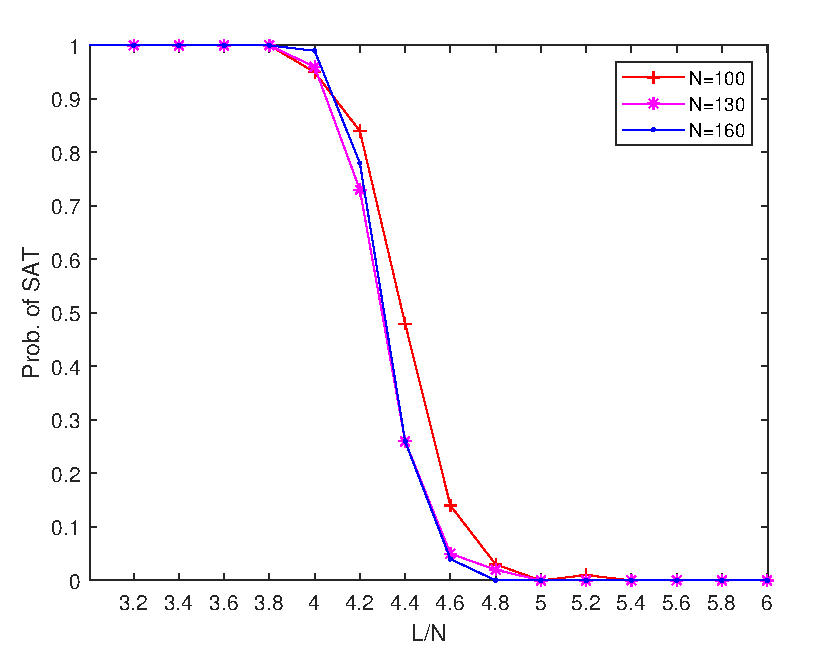
\includegraphics[width=0.5\linewidth]{ProbvsLN}
	\captionsetup{font={scriptsize}}
	\caption{Probability of satisfiability and $L/N$}
	\label{fig:prob-vs-ln}
\end{figure}

\begin{figure}[t]
	\setlength{\leftskip}{0pt}
	\begin{minipage}[t]{0.5\textwidth}
		\centering
		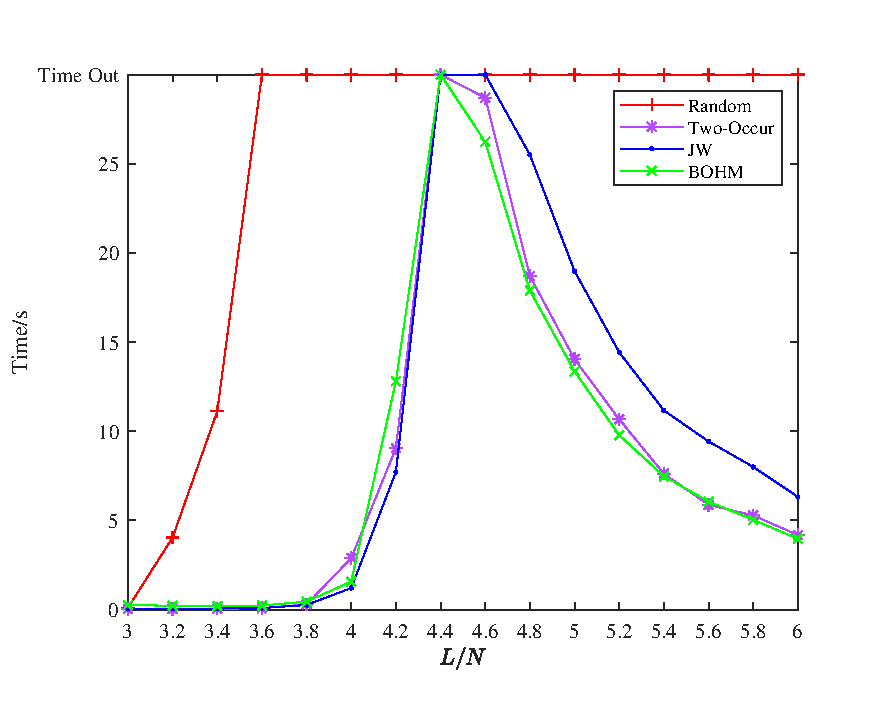
\includegraphics[width=1.1\columnwidth,height=0.72\columnwidth]{TimevsLN}
		\captionsetup{font={scriptsize}}
		\caption{Running time and $L/N$}
		\label{fig:ex-qa}
	\end{minipage}
	\begin{minipage}[t]{0.5\textwidth}
		\centering
		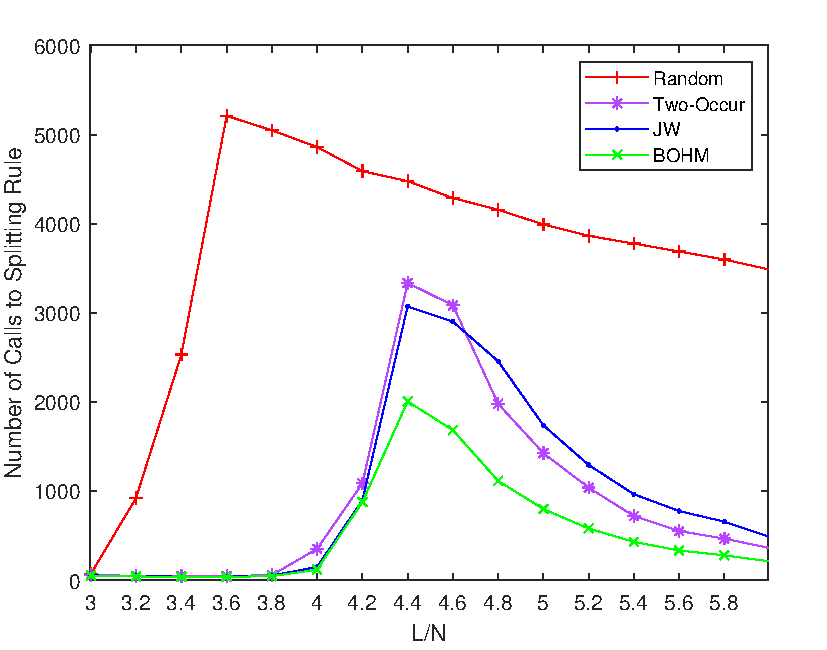
\includegraphics[width=1\columnwidth,height=0.68\columnwidth]{CallsvsLN}
		\captionsetup{font={scriptsize}}
		\caption{Number of calls to splitting rule and $L/N$}
		\label{fig:ex-sm}
	\end{minipage}
\end{figure}



	\subsection{Running time and number of DPLL calls}
	In this section we compare four variable picking heuristics described in 1.3: Random, Two-Occur, Jeroslow-Wang (JW) and BOHM. Due to time limit we set time-out threshold to 30s. We also set $N=160$, which is the largest value of $N$ such that all the  heuristics except random could finish almost all (about 90\%) benchmarks within the time threshold. The number of DPLL calls are counted by the number of spliting rules used. The results of running time are shown in Table 2 and figure 2 while the results of number of DPLL calls are shown in Table 3 and figure 3.
	

	

	\begin{center}
		\begin{table}[th!]
			\resizebox{\textwidth}{13mm}{
			\begin{tabular}{|c|c|c|c|c|c|c|c|c|c|c|c|c|c|c|c|c|}
		\hline 
		$L/N$ & 3.0 & 3.2 & 3.4 & 3.6 & 3.8 & 4.0 & 4.2 & 4.4 & 4.6 & 4.8 & 5.0 & 5.2 & 5.4 & 5.6 & 5.8 & 6.0 \\ 
		\hline 
		Random & 0.10 & 4.04 & 11.12 & TO & TO &TO  & TO & TO & TO & TO & TO & TO & TO & TO & TO & TO \\ 
		\hline 
		Two-Occur& 0.03&0.03&0.05& 0.08 & 0.29 & 2.89 & 9.06 & TO & 28.70 & 18.75 & 14.04 & 10.67 & 7.62 & 5.88 & 5.28 & 4.18   \\ 
		\hline 
		JW &0.06&0.06&0.06& 0.09 & 0.26 & 1.21 & 7.72 & TO & TO & 25.5 & 18.98 &14.43  & 11.17 & 9.43 & 8.00 & 6.32   \\ 
		\hline 
		BOHM & 0.25 & 0.22 & 0.21 & 0.23 & 0.45 & 1.57 & 12.81 & TO & 26.23 & 17.89 &13.36& 9.78 & 7.48 & 6.06 & 5.04 & 3.97   \\ 
		\hline 
	\end{tabular}}
	\captionsetup{font={scriptsize}}
\caption{Running time and $L/N$}
	\end{table}
	\end{center}

	\begin{center}
		\begin{table}[th!]
			\resizebox{\textwidth}{13mm}{
			\begin{tabular}{|c|c|c|c|c|c|c|c|c|c|c|c|c|c|c|c|c|}
		\hline 
		$L/N$ & 3.0 & 3.2 & 3.4 & 3.6 & 3.8 & 4.0 & 4.2 & 4.4 & 4.6 & 4.8 & 5.0 & 5.2 & 5.4 & 5.6 & 5.8 & 6.0 \\ 
		\hline 
		Random & 73 & 927 & 2535 & 5210 & 5048 & 4860 & 4590 & 4478 & 4288 & 4157 & 3992 & 3864 & 3778 & 3689 & 3599 & 3486 \\ 
		\hline 
		Two-Occur & 62 &51  &47  & 49 & 60 & 354 & 1089 & 3336 & 3086 & 1981 & 1427 & 1041 & 722 & 554 & 469 & 363 \\ 
		\hline 
		JW &56  & 50 & 42 & 42 & 55 & 151 & 900 & 3073 & 2902 & 2458 & 1740 & 1295 & 967 & 778 & 659 & 487 \\ 
		\hline 
		BOHM & 54 & 45 & 39 & 40 & 48 & 121 & 879 & 2008 & 1685 & 1117 & 800 & 583 & 432 & 336 & 281 & 214 \\ 
		\hline 
	\end{tabular} }
	\captionsetup{font={scriptsize}}
	\caption{Number of calls to splitting rule and $L/N$}
	\end{table}
	\end{center}

	I will choose BOHM as my heuristic in the following comparasion since it has better performance than JW in hard cases. 
	\subsubsection{Random vs BOHM}
	It's easy to see that BOHM beats Random for  all cases except for the running time on $L/N=3.0$. Since Random ran out of time for at least half of all cases for $L/N\ge3.6$ (that's why the median running time is TO), it's meaningless to show the ratio of runnning time of BOHM to that of Random. However, as shown in Figure 4, we can still draw a plot for ratio of number of calls.

	\subsubsection{Two-Occur vs BOHM}
	To compare the performance of Two-Occur and BOHM, two different heuristics, the ratio of running time of 2-Occur to that of BOHM  is shown in Figure 5 while the ratio of number of calls of splitting rule is shown in Figure 6. 

	\section{Result Analysis}
	\subsection{Influence of L/N}
	From Figure 1 we could see the relation between the probability of satisfability and $L/N$ clearly: for a fixed $N$, when the number of clauses is small ($L/N\le 4$), the probability of satisfability is very close to 1. And when $L/N\ge 4.8$, the probability is fairly close to 0.
	
	The interesting thing is the change of probability from 1 to 0 happens in a small interval ($L/N$ is from 4.0 to 4.8), in other words, the change is so rapid that there is almost no "median state" for probability of satiability.
	
	Theoretical computer scientists have studied this phenonmenon for a long time and called it "phase transition", a jargon first used in physical and chemistry. 
	
	More formally, Friedgut proved that there is a threshold $\alpha_k(N)$ such that for every $\epsilon>0$, a random k-CNF formula with $L/N<\alpha_k(N)+\epsilon$ is SAT w.h.p. (as $N\to \infty$) while if $(L/N>\alpha_k(N)+\epsilon)$ then the random formula is UNSAT w.h.p. 
	
	Whether we can replace $\alpha_k(N)$ to a constant $\alpha_k$ is still an open problem and is conjectured in [5][6][7] based on experimential evidence. For $k=2$ and all sufficient large $k$ the conjecture has been proven  in [8]. However, for small values of $k\ge 3$ the conjecture still remains elusive. For $k=3$, $\alpha_k$ is estimated to be near 4.26 experimentally. From Figure 1 we can see that $\alpha_k$ is between 4.2 and 4.4, which agrees on the well-known estimated value 4.26.
	
	From Figure 1 we could also see the impact of $N$. Comparing the plots of different $N$ one can find that the phase transition of $N=160$ is sharper than those of $N=100$ and $N=130$, which is consistent with the conjecture of cretical ratio $\alpha_k$.
	
	Phase transition has great effect not only on satisfiability of clause but also on the performance of SAT solver, which is highly related with the solution space geometry of CNF formula. For small $L/N$, the solution space is connected w.h.p and the SAT solver can find a solution quickly. And for large $L/N$ the formula is UNSAT w.h.p and SAT solver can realize this fact fast since conflicts happen frequently. However when $L/N$ is in middle, the solution space can be partitioned into many clusters where every cluster is far from  others. This phenonmenon, called "shattering", is known to bring difficulty for a veriety of SAT solvers.\label{key}
	
	From Figure 2 and 3 we can see that the peak of running time and time of calls to splitting rule appears in $[4.4,4.6]$ for all heuristics except Random, which is near the conjecture of $\alpha_k=4.26$. On the other hand, when $L/N$ is far from the peak, the performence of SAT solver is much better.
	
	\subsection{Comparasion of Different Heursitics}	
	Now we will compare the performance of different heuristics from Figure 2 and Figure 3.
	\begin{itemize}
		\item It's obvious that Random has the worst performance: it ran out of time for most values of $L/N$ and it has largest number of calls to splitting rule.
		\item Jeroslow-Wang Heuristics (JW) performed well on easy benchmarks ($L/N$ is small). However when $L/N$ is larger and the time needed for the solver is longer, JW is beaten by Two-Occur and BOHM. Thus I chose BOHM as my heuristic and compare it with Random and Two-Occur in the following.
	\end{itemize} 
	\subsubsection{BOHM vs Random}
		\begin{figure}[h!]
		\centering
		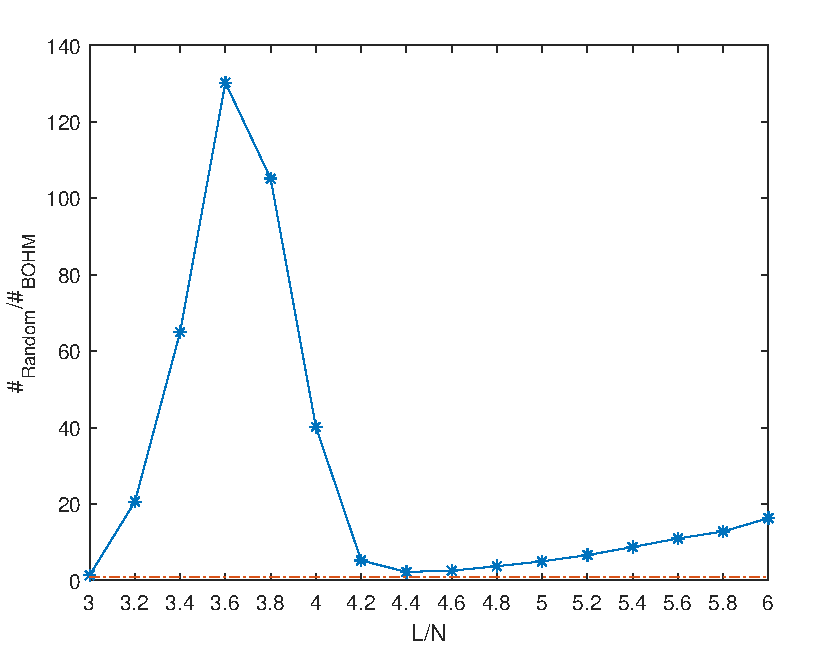
\includegraphics[width=0.5\linewidth]{cRvsB}
		\captionsetup{font={scriptsize}}
		\caption{Ratio of number of calls to splitting rule of Random to BOHM's and $L/N$}
		\label{fig:cRvsB}
	\end{figure}
	The ratio of running time between these two heuristics is somehow meaningless because Random has too many TimeOuts. Thus we will only look at Figure 4 to see the ratio of number of calls to splitting rules. 
	
	When both heuristics did't run out of time ($L/N\le 3.6$), the ratio can be up to 130, meaning that BOHM used much less splitting rules than Random did. And after Random ran out of time ($L/N\ge 3.6$), the ratio decreased because Random didn't actually solve the problem and the number of calls Random used remains the same. Generally speaking, Random is too aimless and not a good choice for variable picking heuristic. 
	\subsubsection{BOHM vs 2-Occur}
		\begin{figure}[t!h]
		\setlength{\leftskip}{0pt}
		\begin{minipage}[t]{0.5\textwidth}
			\centering
			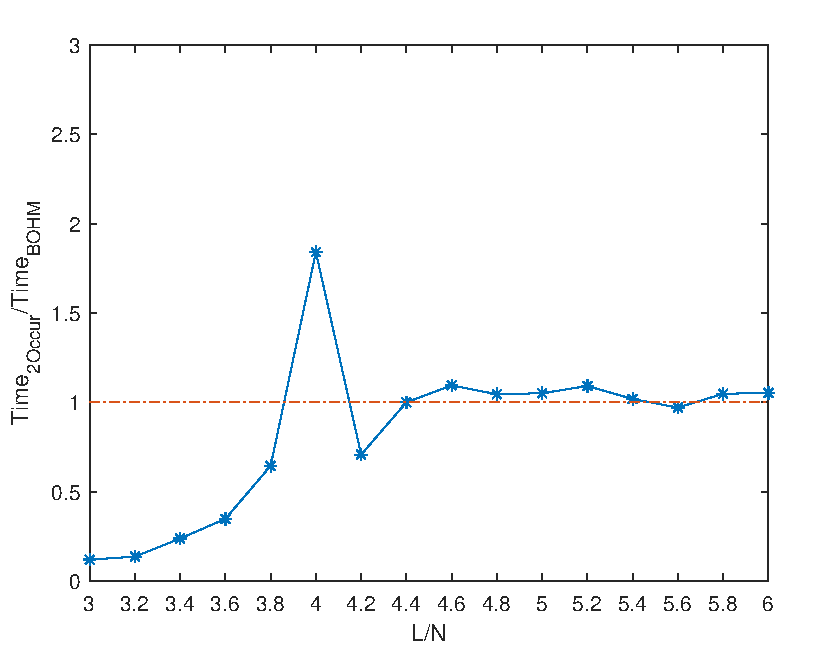
\includegraphics[width=1.0\columnwidth,height=0.785\columnwidth]{tTvsB}
			\captionsetup{font={scriptsize}}
			\caption{Ratio of running time of 2-Occur to BOHM's\\ and $L/N$}
			\label{fig:ex-qa}
		\end{minipage}
		\begin{minipage}[t]{0.5\textwidth}
			\centering
			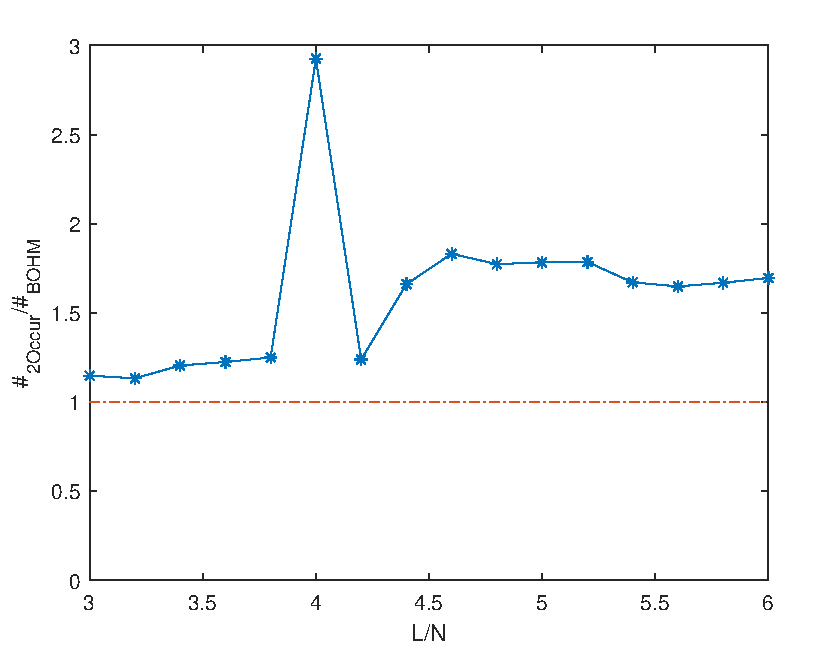
\includegraphics[width=1\columnwidth,height=0.785\columnwidth]{cTvsB}
			\captionsetup{font={scriptsize}}
			\caption{Ratio of number of calls  of 2-Occur to BOHM's and $L/N$}
			\label{fig:ex-sm}
		\end{minipage}
	\end{figure}
	From Figure 5 one can find out that when $L/N$ is small ($L/N\le 3.8$), 2-Occur spent less time than BOHM (this is not very interesting because when $L/N$ is small the actual time the solver needed is less than 0.3s, thus the absolute difference is quite small) while when $L/N\ge 4.4$ BOHM is slightly better, which may imply that BOHM is better at solving hard cases. From figure 3 and Figure 6, this point is more clear: after the peak, BOHM used much less calls compared to other heuristics. 
	
	My interpetation for reason that 2-Occur is better JW is  2-Occur is more greedy while JW puts too much weight on 3-clauses and it turns out 2-clauses are much more important than 3-clauses. Although BOHM also take 3-clauses into consideration, the number of occurance of 3-clause only matters when there is a tie in that of 2-clauses (see the description of BOHM in 1.3). 
	
	Come back to the comparasion of Two-Occur and BOHM. My interpetion  of  figure 6 is besides eliminating clauses, BOHM also pays attentions to reducing more 2-clauses to unit clauses. Thus BOHM have more opportunities doing unit propagation. However why less splitting rules didn't bring corrseponding advantage for BOHM in running time against 2-Occur is still not very straightforward to me.
	\section{Summary}
	\begin{itemize}
		\item Phase transition phenonmenon of random 3-CNF is clearly verfied in the experiments. The critical ratio of number of clauses to that of variables is in $[4.2,4.4]$.
		\item BOHM and 2-Occur performs better than other heuristics considered in the experiments while 2-Occur terminated fast in easy cases ($L/N$ is small) and BOHM used less calls to splitting rules and seemed to do well in hard cases ($L/N$ is large).
	\end{itemize}
	\section{What I Learned From the Project}
	\begin{itemize}
		\item It's so nice to verify the well-known  theory of phase transition. The reason why I like phase transition is because it is very similiar to a physical phenmenon, which really exists, appears in very fundamental problems, is easy to observe by everyone and is probably invariant with the development of techniques. 
		\item I have never done  such time-consuming experiments like this project. I realized many coding habits I used to have can waste a lot of time and prevent me from handling a large experiment. From this project I learned how to estimate the time needed for the experiment,  choose  appropriate experiment parameters and separate the code of algorithm and experiments.
		\item I should have started the project earlier so that I would have more time for running the experiment and could use large $N$ to get nicer results.
	\end{itemize}


\renewcommand\refname{Reference}
\bibliographystyle{plain} \bibliography{Thesis} 

[1] Carsten Sinz, Tomáš Balyo. Practical SAT Solving Lecture 5, Kalsruhe Institute of Technology

[2] Joao Marques-Silvam, The Impact of Branching Heuristics in Propositional Satisfiability Algorithms

[3] M. Buro and H. Kleine-B¨uning. Report on a SAT competition. Technical report,
University of Paderborn, November 1992.

[4] The Hard Problems Are Almost Everywhere For Random CNF-XOR Formulas 

[5] David Mitchell, Bart Selman, and Hector
Levesque. Hard and easy distributions of SAT problems. In Proc.
of AAAI, pages 459–465, 1992.

[6] James M. Crawford and Larry D. Auton. Experimental results on the crossover point in satisfiability
problems. In Proc. of AAAI, pages 21–27, 1993.

[7] Scott Kirkpatrick and Bart Selman. Critical behavior in the satisfiability of random boolean
expressions. Science, 264(5163):1297–1301, 1994

[8]Jian Ding, Allan Sly, and Nike Sun. Proof of
the satisfiability conjecture for large k. In Proc. of SToC, pages
59–68, 2015.
\end{document}
